%!TeX program = xelatex

\documentclass[aspectratio=169]{beamer}
\usepackage[main=russian,english]{babel}

\usepackage{fontspec}
\usepackage{graphicx}
\usepackage{xcolor}
\usepackage{xltxtra}
\usepackage{hyperref}
\usepackage{multicol}
\usepackage{unicode-math}
\usepackage{changepage}

\usepackage{tcolorbox}
\tcbuselibrary{skins}

\setmainfont{Iosevka NFM}
\setmonofont{Iosevka NFM}
\setsansfont{Iosevka NFM}
\setromanfont{Iosevka NFM Italic}
%\setmathfont{DejaVu Math TeX Gyre}
\setmathfont{Latin Modern Math}


\title{Планировщик процессов для гетерогенных процессорных архитектур}
\author{Шаго Павел Евгеньевич}
\institute {
        Научный руководитель: Корхов Владимир Владиславович \\
        \vspace{0.5cm}
        Факультет прикладной математики -- процессов управления\\
        Кафедра моделирования электромеханических и компьютерных систем
}

\usetheme{Warsaw}

\newtcolorbox{shadowbox}{
  enhanced,
  colback=white,
  colframe=white,
  boxrule=0pt,
  sharp corners=all,
  arc=6pt,
  drop shadow,
  left=4mm,
  right=4mm,
  top=2mm,
  bottom=2mm
}

\begin{document}


\begin{frame}
        \titlepage
\end{frame}


\begin{frame}
        \frametitle{Цель и задачи}

        \begin{block}{Цель}
                Разработать более эффективный планировщик процессов
                для гетерогенного процессора (aka Hybrid CPU, big.LITTLE)
        \end{block}
        
        \begin{block}{Задачи}
                \begin{itemize}
                        \item Переписать EEVDF на sched\_ext
                \end{itemize}
        \end{block}

\end{frame}


\begin{frame}
       Тут будет обоснование почему это не очень хорошо для ARL,
       как это можно было бы поправить с точки зрения алгоритма
       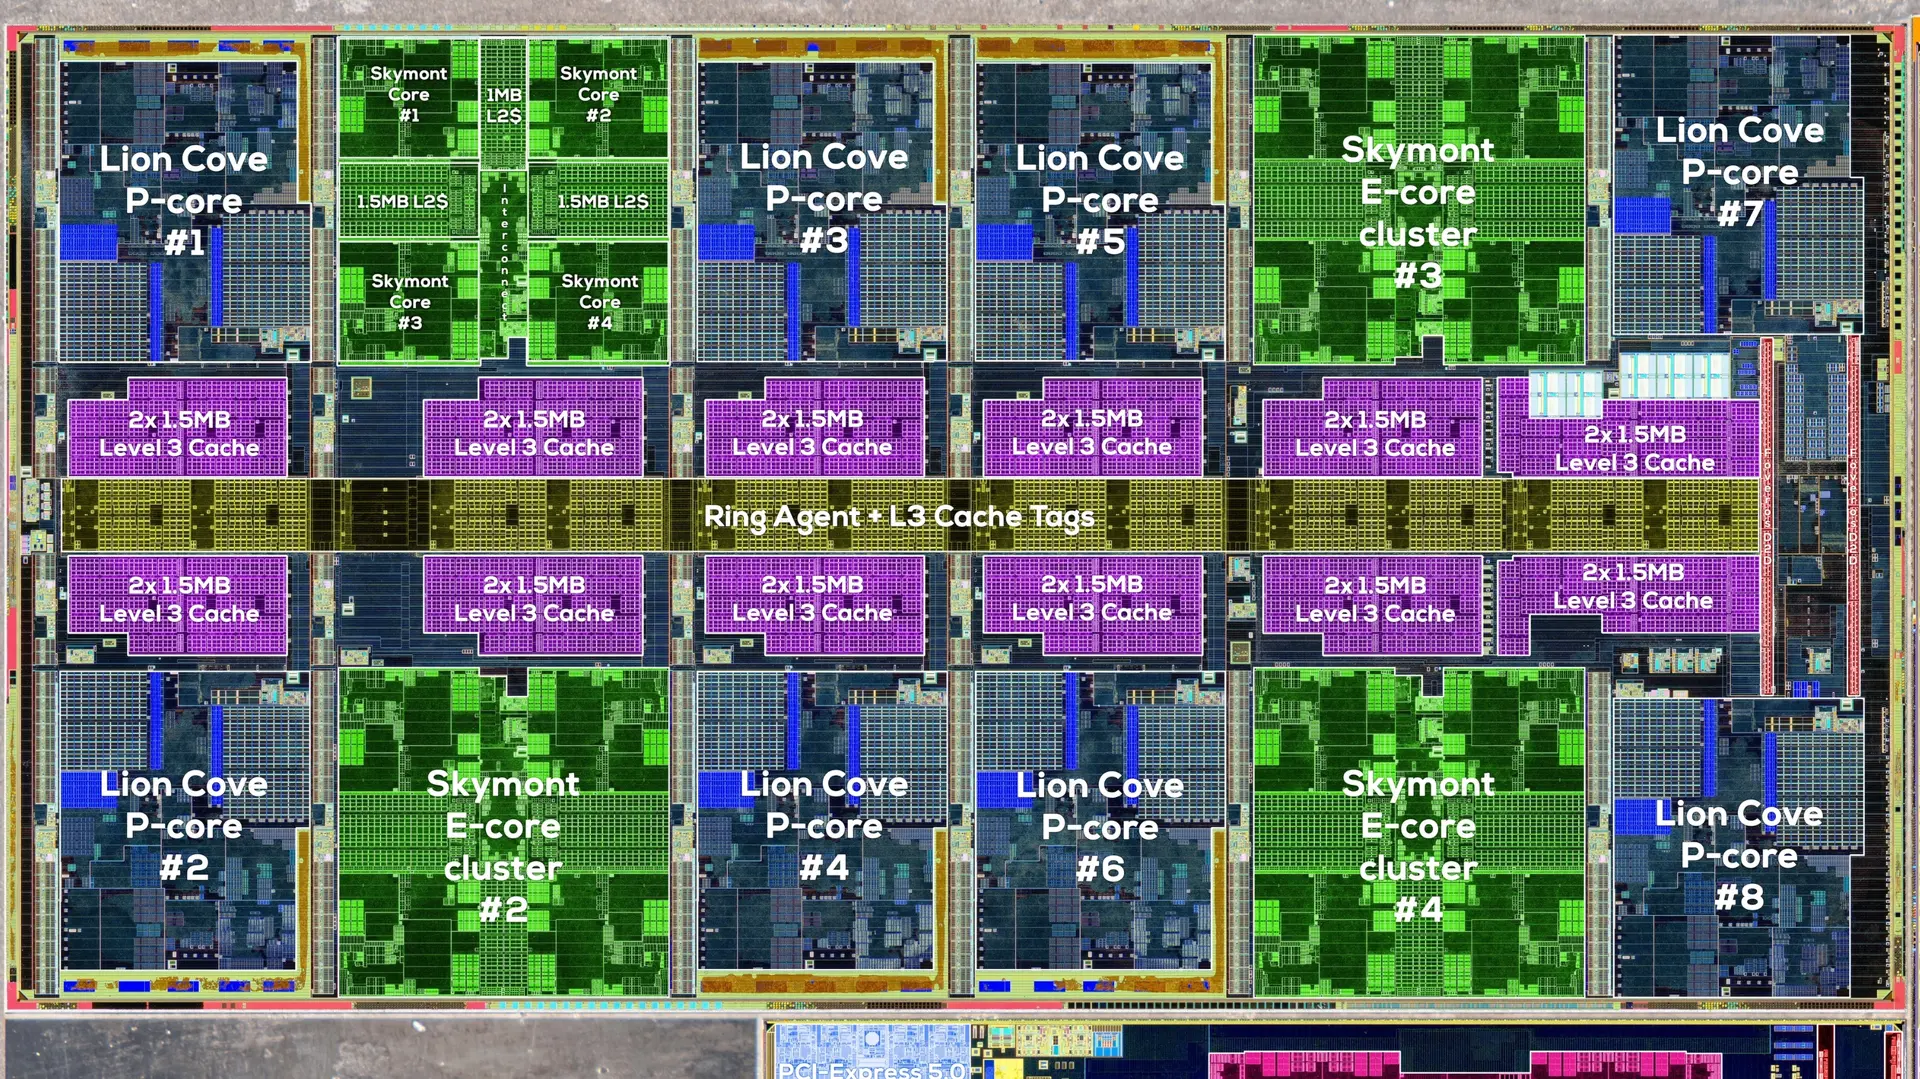
\includegraphics[width=0.85\linewidth]{res/ARL.png}
\end{frame}


\begin{frame}
        \frametitle{Введение}

        \begin{itemize}
                \item Алгоритм построен на концепции сведения параметров задачи
                        в одну функцию -- виртуальное время.
                \item Решение о планировании принимается так: выбирается процесс
                        у которого есть доступный запрос с самым ранним
                        виртуальным дедлайном.
                \item Главный результат: гарантия справедливости алгоритма
                        EEVDF, задержка строго ограничена размером временного
                        кванта $ q $.
                \item Показано, что ограничение является оптимальным для алгоритмов
                        пропорционального распределения и улучшает все предыдущие ограничения.
        \end{itemize}

        \begin{shadowbox}
        Earliest Eligible Virtual Deadline First : A Flexible
        and Accurate Mechanism for Proportional Share Resource Allocation

        \vspace{0.2cm}
        Ion Stoica, Hussein Abdel-Wahab

        Old Dominion University 1996
        \end{shadowbox}

\end{frame}




\begin{frame}
        \frametitle{Предположения}

        \begin{itemize}
                \item Процессы конкурируют за общий разделяющийся по времени
                        ресурс (CPU).
                \item Ресурс распределяется во временных квантах не больше чем
                        $ q $.
                \item В начале каждого кванта времени для использования ресурса
                        выбирается процесс.
                \item После того как процесс захватил ресурс он может
                        использовать его весь квант времени либо освободить до
                        окончания кванта времени.
                \item Каждому процессу назначается вес $ w_i $ определяющий 
                        относительную долю времени которая ему положена.
                \item Только процессы могут порождать временные кванты.
        \end{itemize}

\end{frame}


\begin{frame}
        1. Доля клиента (Client Share, $f_i(t)$)
        Доля ресурса, которую клиент $i$ должен получить в момент времени $t$, определяется отношением
        его веса ($w_i$) к сумме весов всех активных клиентов ($A(t)$):
        $$f_i(t) = \frac{w_i}{\sum_{j \in A(t)} w_j}$$
\end{frame}


\begin{frame}
        Тут будут результаты работы
\end{frame}


\begin{frame}
        Тут будет короткое напоминание что такое eBPF и shed\_ext
\end{frame}



\begin{frame}
        Сведения о реализации, сравнительный график EEVDF (sched\_ext)
        vs EEVDF
\end{frame}


\begin{frame}
        \frametitle{Спасибо за внимание, вопросы?}
        
        \large Репозиторий с реализацией

        \begin{adjustwidth}{2cm}{0cm}
                \begin{thebibliography}{20}
                        \bibitem{paper}
                        \href{https://github.com/shgpavel/A1349}
                        {https://github.com/shgpavel/A1349}
                \end{thebibliography}
        \end{adjustwidth}

        \vspace{1.4cm}
        \large Репозиторий с другими scx планировщиками

        \begin{adjustwidth}{2cm}{0cm}
                \begin{thebibliography}{20}
                        \bibitem{paper}
                        \href{https://github.com/sched-ext/scx}
                        {https://github.com/sched-ext/scx}
                \end{thebibliography}
        \end{adjustwidth}

\end{frame}


\begin{frame}
        \frametitle{Дополнительный слайд. Обозначения}
        $ n $ -- количество процессов

        \vspace{0.03cm}
        $ n_a $ -- количество активных процессов

        \vspace{0.03cm}
        $ w_i $ -- вес $ i $-го процесса

        \vspace{0.03cm}
        $ q $ -- квант времени

        \vspace{0.03cm}
        $ m $ -- количество выделенных временных квантов

        \vspace{0.03cm}
        $ r $ -- запрошенное процессом время на исполнение

        \vspace{0.03cm}
        $ r_{max} $ -- максимально возможное время на исполнение

        \vspace{0.03cm}
        $ r_i^{(k)} $ -- продолжительность исполнения $ k $-го запроса $ i $-го
        процесса

        \vspace{0.03cm}
        $ u_i^{(k)} $ -- время которое фактически получает процесс $ i $ на
        k-ом запросе

        \vspace{0.03cm}
        $ t $ -- момент в реальном времени

        \vspace{0.03cm}
        $ t_a $ -- момент реального времени когда процесс $ i $ становится
        активным

        \vspace{0.01cm}
        $ t^{-} $ -- время прямо перед наступлением события

        \vspace{0.01cm}
        $ t^{+} $ -- время сразу после наступления события
        
        \vspace{0.01cm}
        $ A(t) $ -- множество всех активных в момент $ t $ процессов

        \vspace{0.01cm}
        $ W(t) $ -- сумма весов всех активных процессов

\end{frame}


\begin{frame}
        \frametitle{Дополнительный слайд. Обозначения}
        \vspace{0.03cm}
        $ f_{i}(t) $ -- доля процесса $ i $ во время $ t $
        
        \vspace{0.03cm}
        $ S_{i}(t_0, t_1) $ -- время обслуживания которое должен получить
        процесс $ i $ в идеальной системе

        \vspace{0.03cm}
        $ s_{i}(t_a, t) $ -- время обслуживания которое клиент $ i $ на
        самом деле получает

        \vspace{0.03cm}
        $ V(t) $ -- виртуальное время системы

        \vspace{0.03cm}
        $ e $ -- реальное подходящее время время запроса
        
        \vspace{0.03cm}
        $ d $ -- реальный дедлайн запроса

        \vspace{0.03cm}
        $ B $ -- множество активных процессов дедлайн которых в $ [e, d] $

        \vspace{0.03cm}
        $ C $ -- множество активных процессов дедлайн которых больше $ d $

        \vspace{0.03cm}
        $ ve_i^{(k)} $ -- виртуальное подходящее время $ k $-го запроса $ i $-го
        процесса

        \vspace{0.03cm}
        $ vd_i^{(k)} $ -- виртуальный дедлайн $ k $-го запроса $ i $-го
        процесса

        \vspace{0.03cm}
        $ lag_{i}(t) $ -- задержка обслуживания процесса $ i $ в момент
        времени $ t,\ (S - s) $ 

        \vspace{0.03cm}
        $ d_{neg} $ -- наибольший дедлайн среди всех процессов с отрицательными
        $ lag $ которые активны в момент времени $ t_1 $

\end{frame}



\end{document}
